%%%%%%%%%%%%%%%%%%%%%%%%%%%%%%%%%%%%%%%%%%%%%%%%%%%%%%%%%%%%%%%%%%%%%%%%%%%%%%%
\subsection{Functional Groups within the Colony}
%%%%%%%%%%%%%%%%%%%%%%%%%%%%%%%%%%%%%%%%%%%%%%%%%%%%%%%%%%%%%%%%%%%%%%%%%%%%%%%

The leading eigenvector (LE) community detection algorithms revealed two communities with a similar size (modularity score of 0.25). The walktrap algorithm (WT) discovered three communities instead, also evenly distributed (modularity score of 0.23). Table~\ref{tab:n3-communities} lists the precise number of members per community and algorithm for snapshot~3.

For both algorithms the communities correspond to different age groups. For LE, the average age of the young community is $13.2$ days, and for the old community $28.7$ days. For WT, the average age of the young community is $6.6$ days and $29.3$ days for the older commmunity. The third middle-aged community of WT is on average 25.1 days old. The age distribution for each algorithm is represented in figure~\ref{fig:n3ageLE} and~\ref{fig:n3ageWT}. The two sample Kolmogorov-Smirnov test confirmed that the age distributions per community are significantly different. The corresponding $p$-values are listed in table~\ref{tab:n3-pvalues2}.

Each community occupies a different region of the comb.
Figure~\ref{fig:n3-communities} shows that the young communities spend the most time in the comb center and the old communities closer to the hive exit. The middle-aged community is positioned between the young and old community and in the periphery of the comb.

\begin{table}[htb]
\small
\centering
\caption[Communities per algorithm]{\textbf{Communities per algorithm} Communities marked with * contain the queen. Age and standard deviation (SD) are measured in days. The queen and nine bees with a negative age are excluded from this analysis.}
\label{tab:n3-communities}
\vspace*{5mm}
\begin{tabular}{lcrrrrr}
	\toprule
	{}  & Community ID & Members & Proportion & Age & SD\\
	\midrule  
	\quad LE  & CY & $*381$  & 41.78\% & $13.15$ & $\pm13.50$ \\
	          & CO & $531$   & 58.22\% & $28.70$ & $\pm11.67$ \\
    \midrule 
	\quad WT & CY & $*229$  & 25.11\% & $6.55$  & $\pm10.36$\\
			 & CM & $298$  & 32.68\% & $25.08$ & $\pm11.97$\\
			 & CO & $385$  & 42.21\% & $29.29$ & $\pm11.44$\\
	\bottomrule
\end{tabular}
\end{table}
\begin{table}[htb]
\small
\centering
\caption[Kolmogorov-Smirnov test]{\textbf{Kolmogorov-Smirnov test} $p$-values for leading eigenvector (LE) and walktrap (WT)}
\label{tab:n3-pvalues2}
\vspace*{5mm}
\begin{tabular}{crrrrr}
	\toprule
	 Communities & LE p-value & WT p-value\\
	\midrule 
    CY, CO & 5.10e-66 & 5.51e-67\\
    CY, CM &          & 1.10e-95\\
    CM, CO &          & 1.98e-05\\ 
	\bottomrule
\end{tabular}
\end{table}

\begin{figure}[!htb]
	\centering
	\begin{subfigure}[b]{1.0\textwidth}
	\centering
	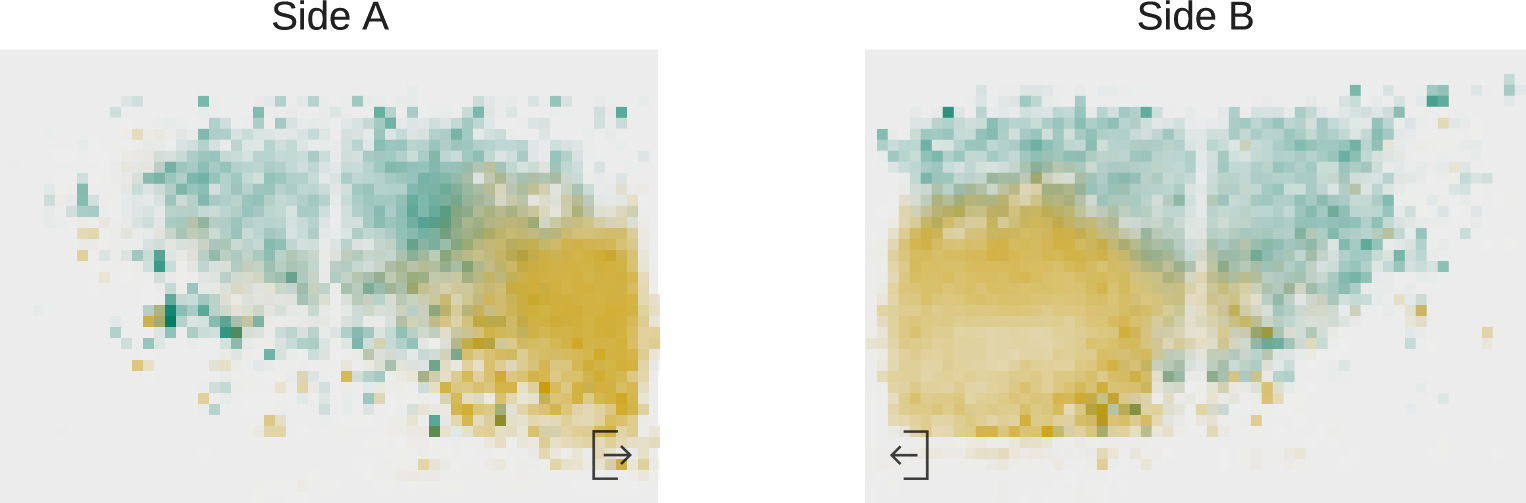
\includegraphics[width=1.0\textwidth]{Figures/le_network3}
	\end{subfigure}
	
	\begin{subfigure}[b]{1.0\textwidth}
	\centering
	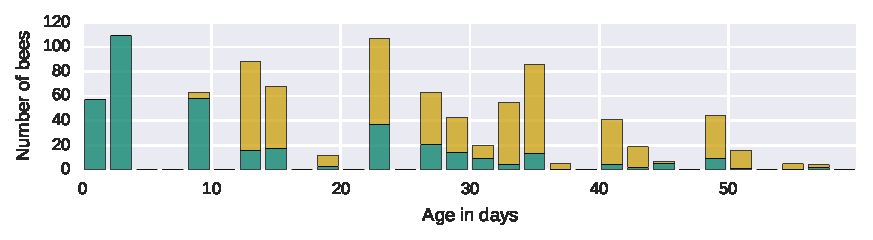
\includegraphics[width=1.0\textwidth]{Figures/n3-ageDistribution-LE}
	\caption[Leading eigenvector communities]{Leading eigenvector communities}
	\label{fig:n3ageLE}
	\end{subfigure}
	
	
	
	\begin{subfigure}[b]{1.0\textwidth}
	\vspace{1pt}
	\centering
	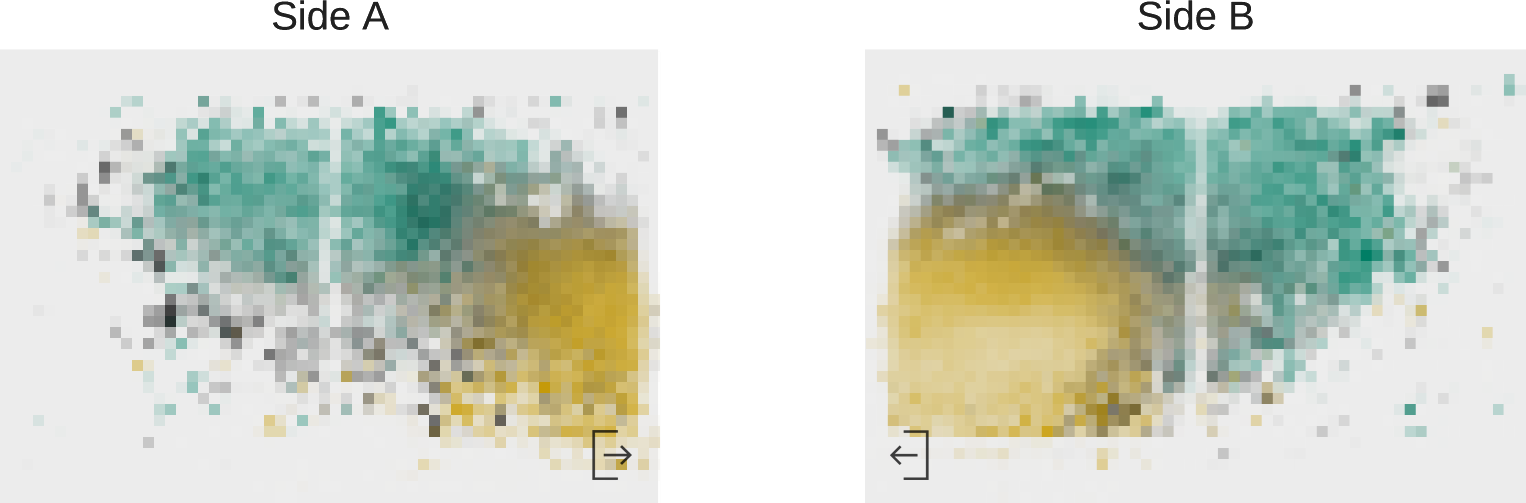
\includegraphics[width=1.0\textwidth]{Figures/wt_network3}
	\end{subfigure}
	
	\begin{subfigure}[b]{1.0\textwidth}
	\centering
	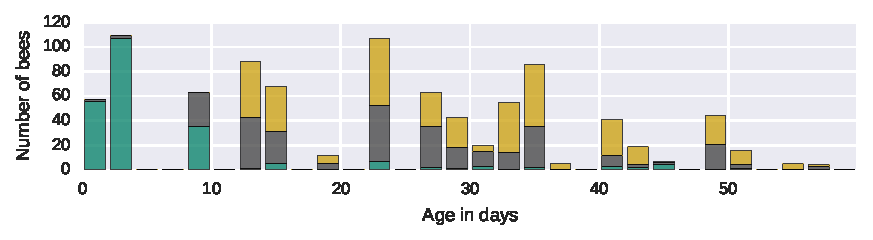
\includegraphics[width=1.0\textwidth]{Figures/n3-ageDistribution-WT}
	\caption[Walktrap communities]{Walktrap communities}
	\label{fig:n3ageWT}
	\end{subfigure}
	
	
	\caption[Age and spatial distribution of communities]{\textbf{Age and spatial distribution of communities} \emph{Green} represents the young community occupying the center area of the comb and \emph{orange} the old community, which is situated closer to the hive access. For walktrap the \emph{gray} middle-aged community is positioned between the other to and in the periphery of the comb.}
	\label{fig:n3-communities}
\end{figure}